\documentclass[]{report}[12 pt]
\usepackage{geometry}
\usepackage{amsmath}
\usepackage{graphicx}
\usepackage{hyperref}
\geometry{margin= 1.5 cm}
\begin{document}
	\begin{titlepage}
	\begin{center}
		\vspace*{1cm}
		
		\Huge
		\textbf{Laboratory Report}
		
		\vspace{0.5cm}
		\LARGE
		X Ray Diffraction\\
		\vspace{0.5cm}
		\textbf{Guide: Prof. Sangita Bose}
		
		\vspace{1.5cm}
		
		\textbf{A R Bathri Narayanan}\\
		Roll no: P0211501\\
		UM DAE Centre for Excellence in Basic Sciences
		
		\vspace{3 cm}
		
		Report presented for the\\
		Advanced Physics Laboratory Course (PL 701)
		
		\vspace{0.8cm}
		
		
\includegraphics[width=0.4\textwidth]{cebs.jpg}
		
		\Large
		School of Physical Sciences\\
		UM-DAE Centre for Excellence in Basic Sciences\\
		Mumbai, MH, India\\
		\today
		
	\end{center}
\end{titlepage}
	\section*{Objectives:}
	\begin{enumerate}
		\item To understand the concept of a Lock-In amplifier and apply it to a simple electronics problem.
		\item To find the critical temperature of the given material using a cooling source (Liquid He is used)
	\end{enumerate}
	\section*{Apparatus required:}
     Lock-In amplifier, Coil, Superconducting setup etc.
     \begin{center}
     	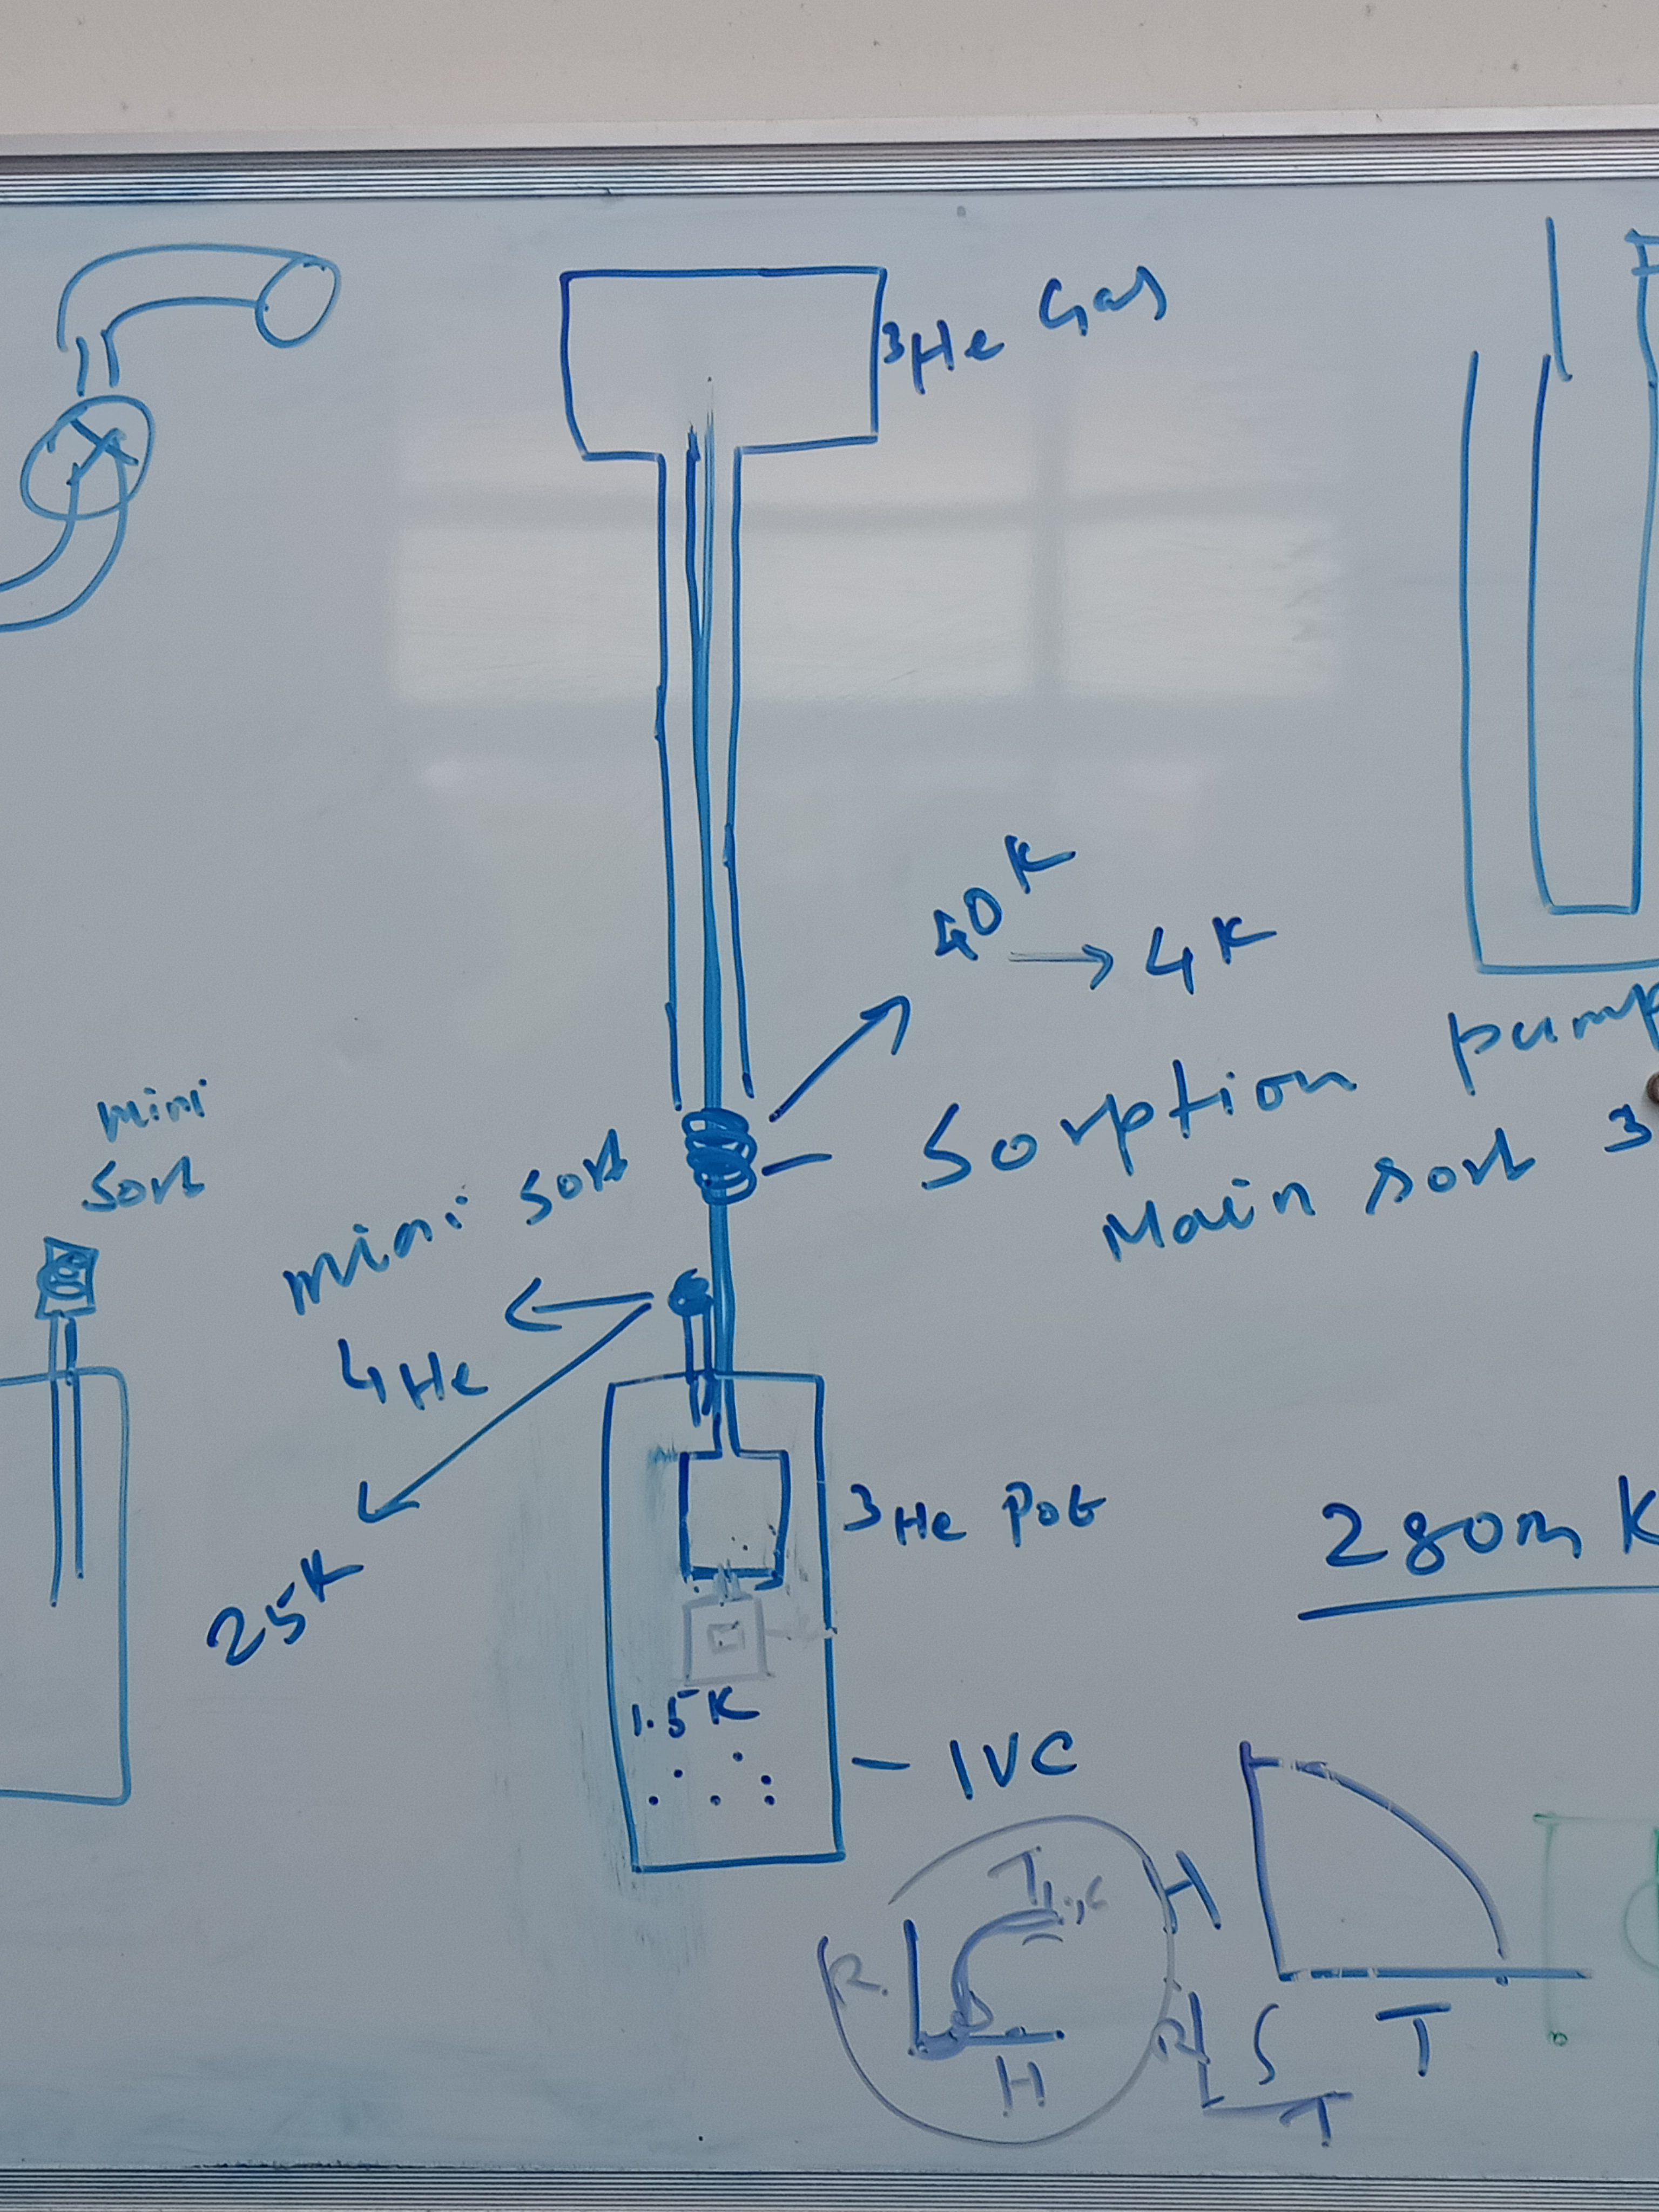
\includegraphics[width=5 cm]{lia5.jpg}
     	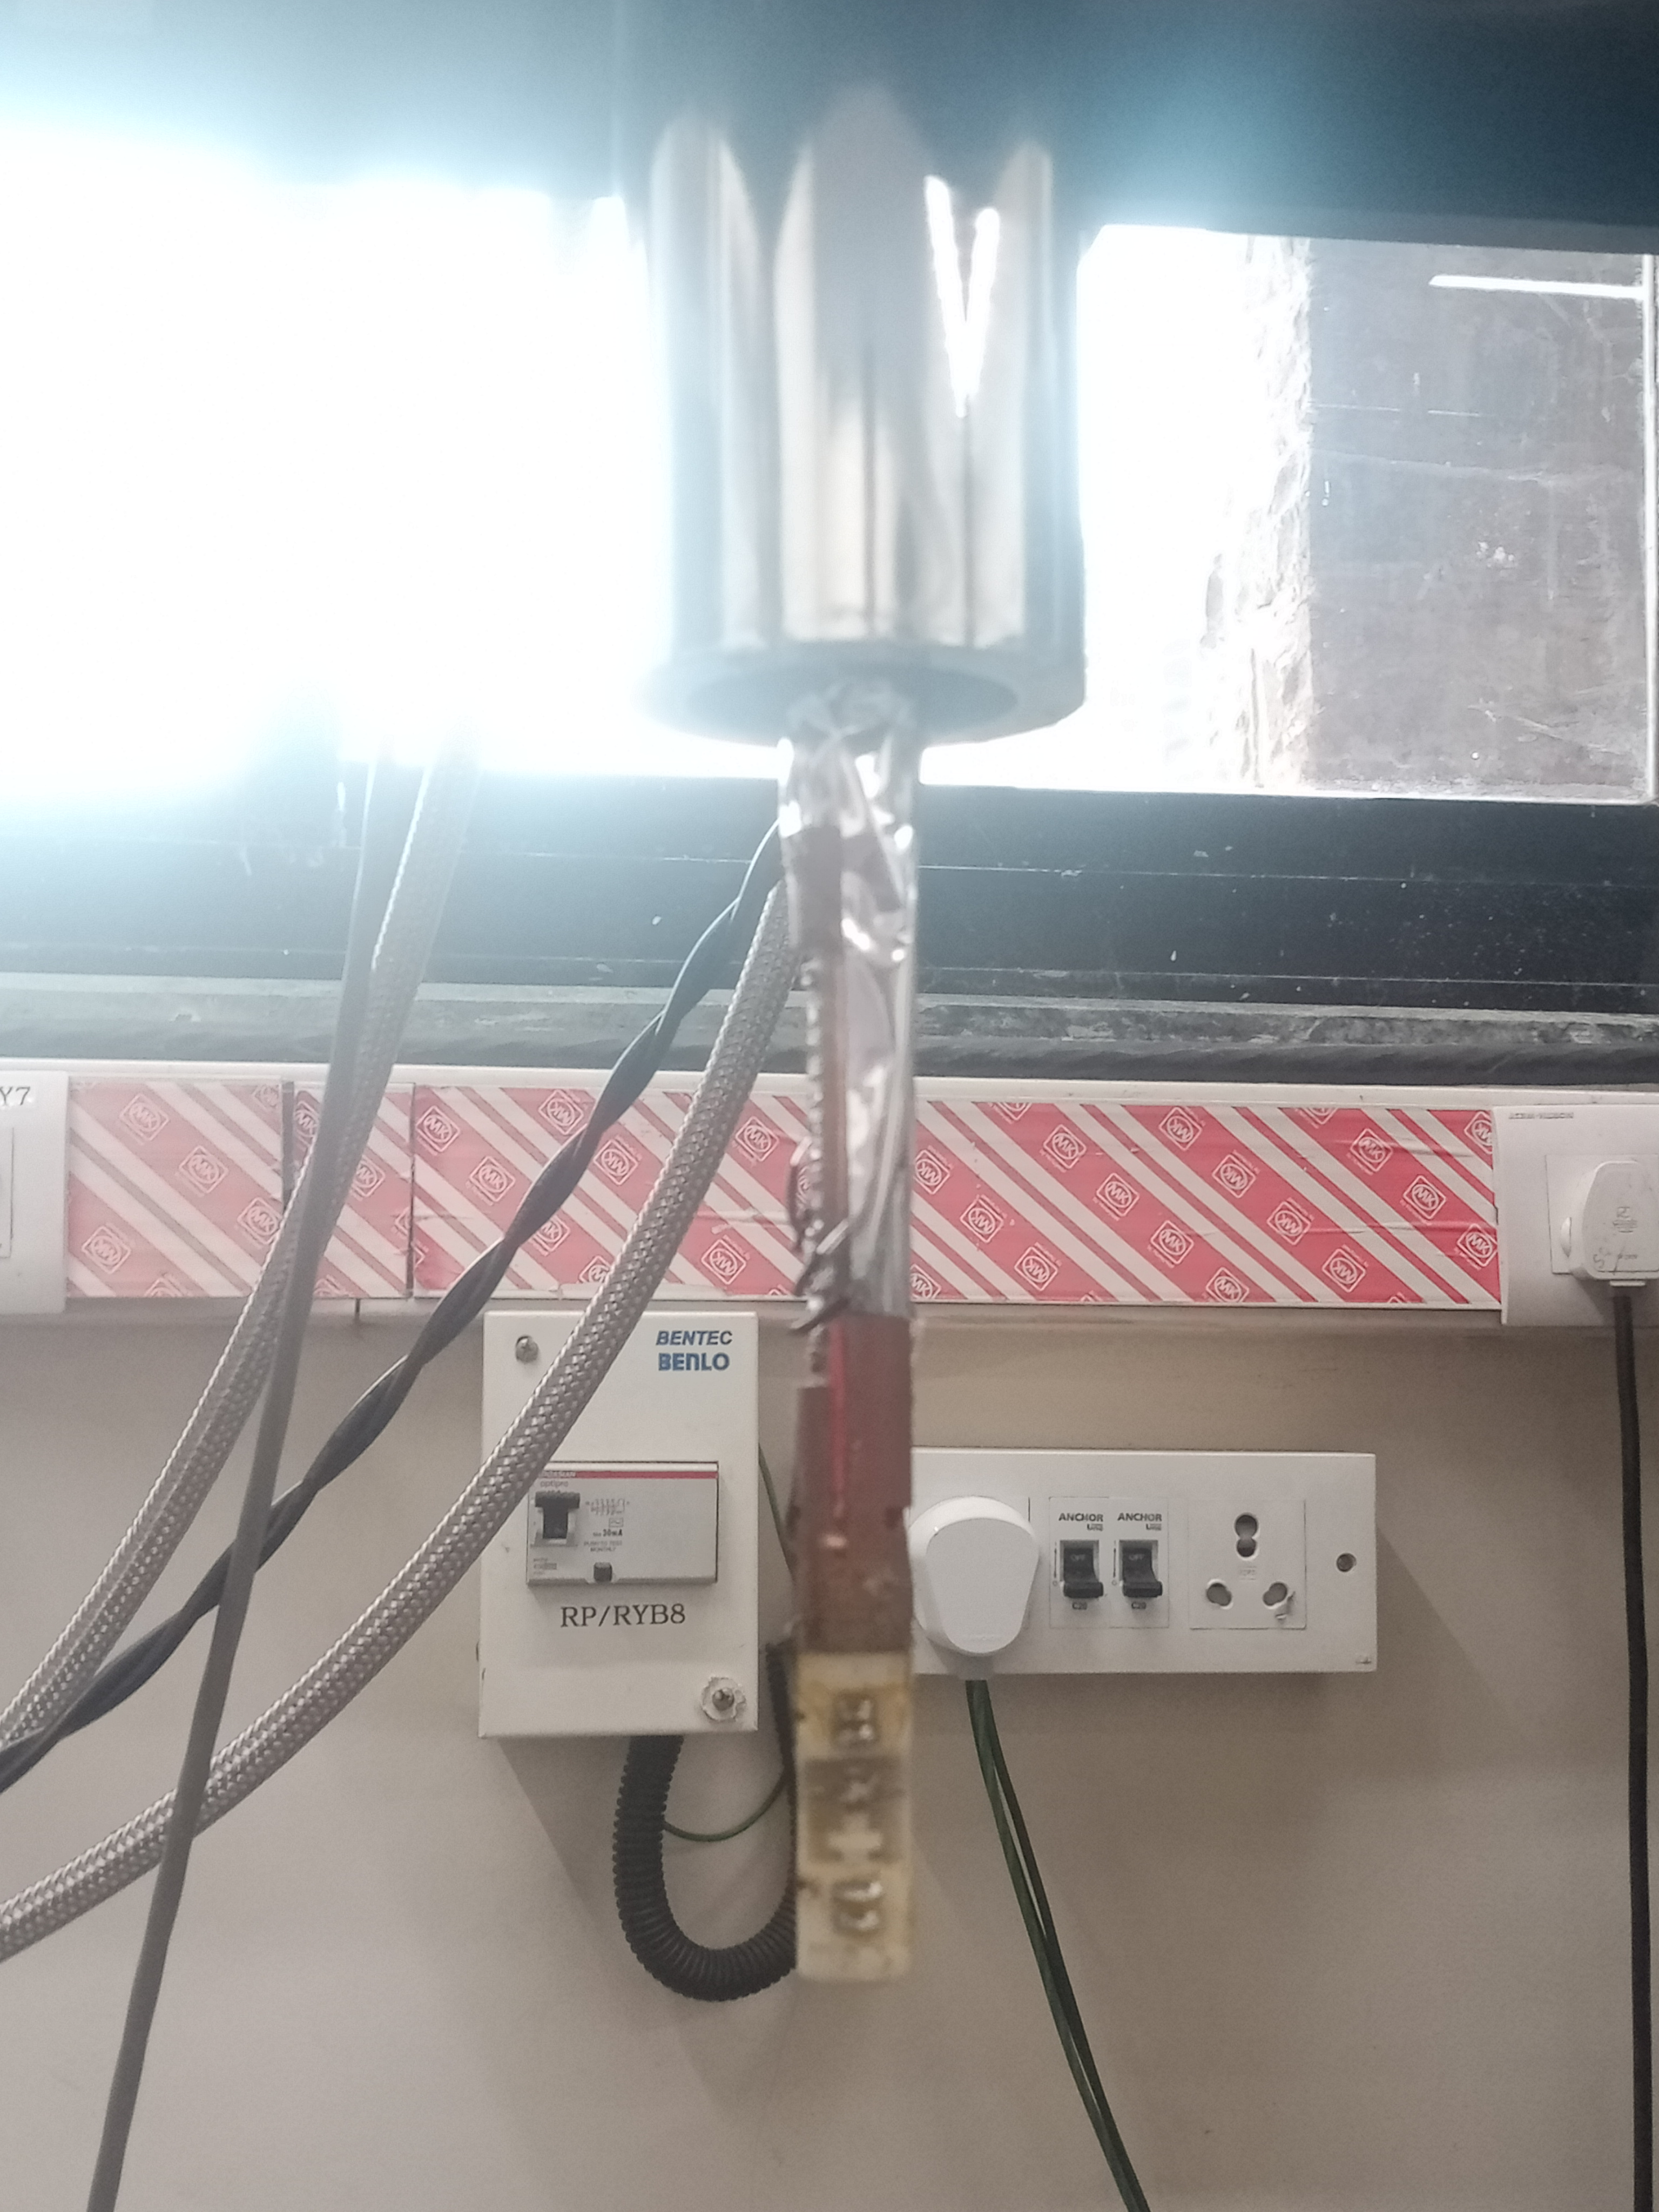
\includegraphics[width=5 cm]{lia6.jpg}\\
     	The schematic and actual setup of the experiment
     \end{center}
	\section*{Theory:}
A lock-in amplifier can identify and analyze extremely tiny AC signals, as low as a few nanovolts, even when they are masked by noise sources that are millions of times larger. It isolates the signal component at a certain reference frequency and phase using a method known as phase-sensitive detection.
Typically, lock-in amplifiers use a phase-locked loop (PLL) locked to an external frequency reference $\omega$  to create their own internal reference signal.
\begin{center}
	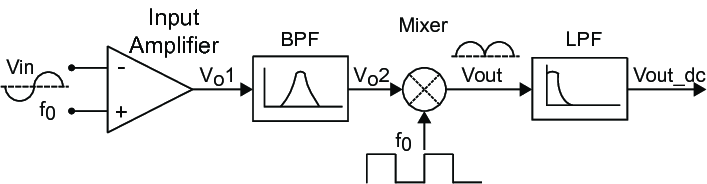
\includegraphics[width=10cm]{lia1.png}\\
	Block diagram of a Lock-In amplifier\\
	\vspace{1 cm}
		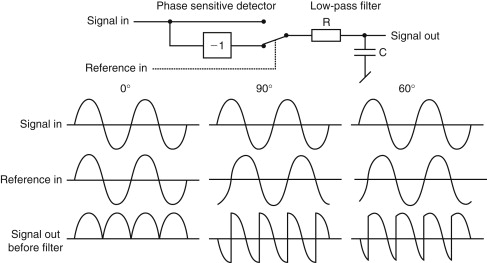
\includegraphics[width=10cm]{lia2.jpg}\\
		Signal processing of a Lock-In amplifier\\
		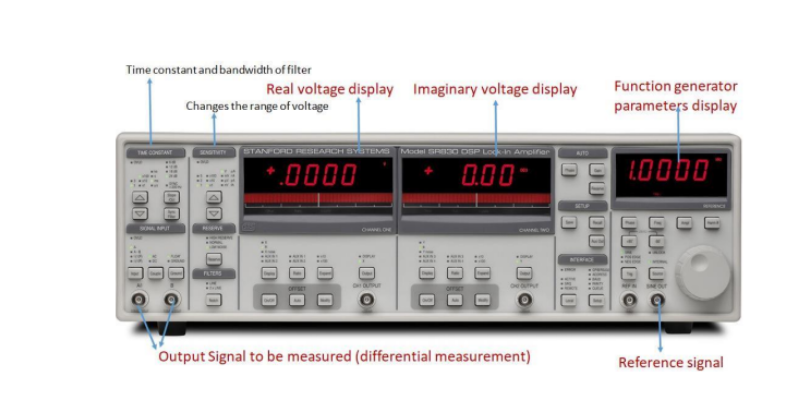
\includegraphics[width=13cm]{lia3.png}\\
		Labeling of our Lock-In amplifier
\end{center}
\textbf{Parameters:}
\begin{align*}
	\text{In phase component}&=V_0cos\theta \\
	\text{Out of phase component}&=V_0sin\theta \\
	\text{Magnitude of signal}&=V_0\\
	\text{Phase}&=arctan\big(\frac{Y}{X}\big)
\end{align*}
\begin{center}
	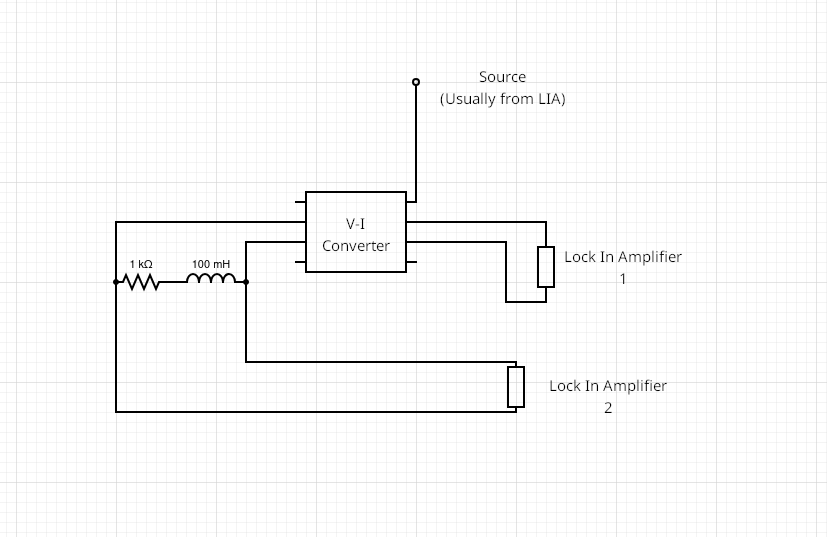
\includegraphics[width=10cm]{lia4m.png}\\
	Schematic diagram of the wire connections. Note that Lock In Amplifiers 1 and 2 are connected, and the terminals of the LIA are actually the A and B channels.
\end{center}
	\section*{Observations:}
\subsection*{Finding the Resistance and Inductance of the given coil}
We have the following data 
\begin{center}
	\begin{tabular}{|c|c|c|c|c|c|c|}
		\hline
		Frequency (Hz)  & Phase 1 (mV) & Voltage 1 Re (mV) & Voltage 1 Im (mV) & Voltage 2 Re($\mu$V) & Voltage 2 Im($\mu$V) & Phase 2 \\
		\hline
		200 & -179.98 & 5.082 & 0 & 147.85 & 0 & 13.32 \\
		\hline
		400 & -179.98 & 5.081 & 0 & 148.38 & -18.1 & 13.29 \\
		\hline
		600 & -179.98 & 5.081 & 0.007 & 148.4 & -21.9 & 13.29 \\
		\hline
		800 & -179.98 & 5.08 & 0.01 & 148.27 & 23.3 & 13.29 \\
		\hline
		1000 & -179.98 & 5.08 & 0.014 & 148.3 & 23.51 & 13.29 \\
		\hline
		1200 & -179.98 & 5.08 & 0.018 & 148.44 & 23.3 & 13.29 \\
		\hline
		1400 & -179.98 & 5.082 & 0.018 & 148.87 & 22.81 & 13.29 \\
		\hline
		1600 & -179.98 & 5.082 & 0.021 & 149.09 & 22.11 & 13.29 \\
		\hline
		1800 & -179.98 & 5.081 & 0.021 & 149.34 & 21.34 & 13.29 \\
		\hline
		2000 & -179.98 & 5.081 & 0.024 & 149.59 & 20.45 & 13.29 \\
		\hline
	\end{tabular}
\end{center}
Where 1 indicates the Lock-In Amplifier linked to the converter and 2 indicates the Lock-In Amplifier linked to the coil. We get the current to be 0.5082 mA.
So the resistance of the coil is 
\[R_{coil}=\frac{Voltage(Real)\text{   }2}{Current}=0.292 \pm 0.001  \Omega \]
Inductance can be found out by plotting the Voltage 2 (Imaginary) with Frequency and getting the slope.
\begin{center}
	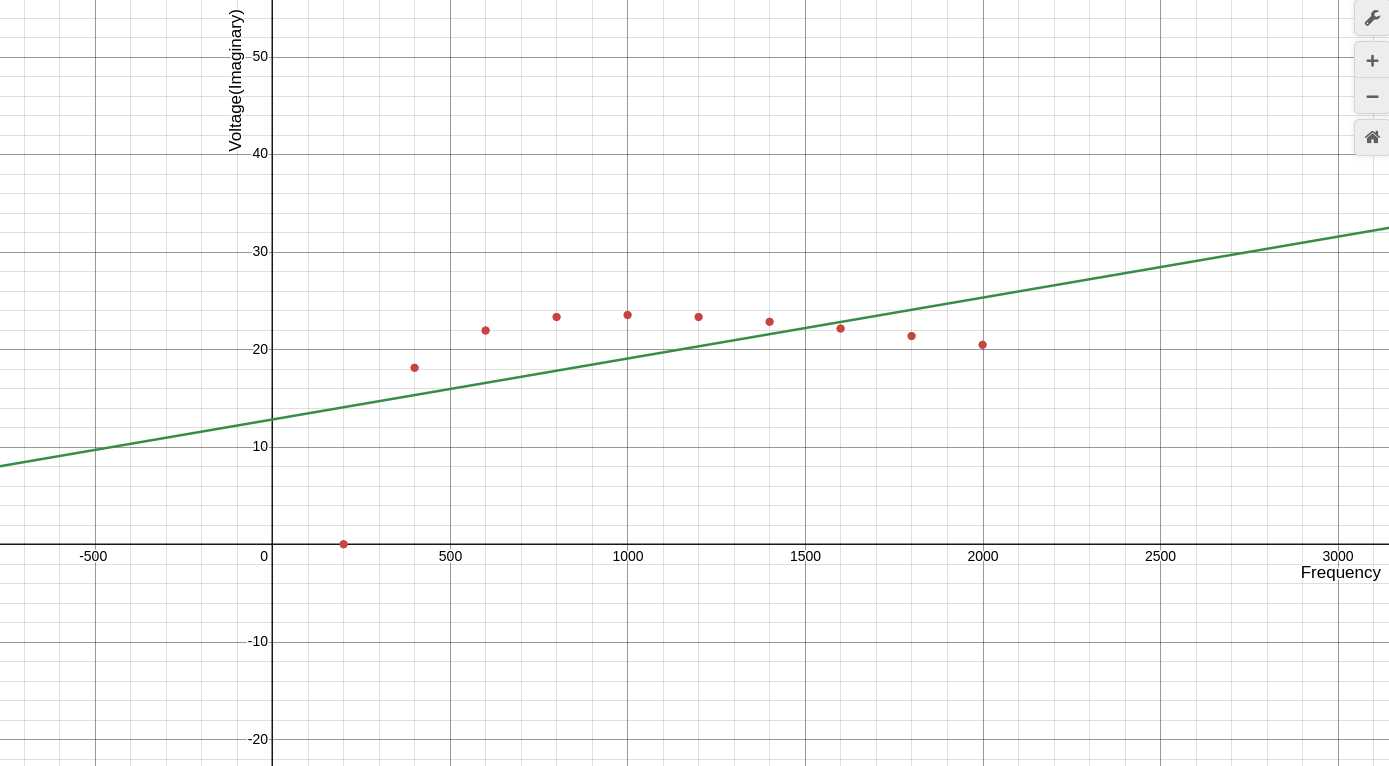
\includegraphics[width=10 cm]{ind.png}
\end{center}
We have the slope=L*I=0.0062$\pm$0.0035
\[\implies L = \frac{0.0062}{I}=12 \mu H\]
Error in Inductance =6.7 $\mu$ H\\
The reason for the high error value is due to the fact that as we go to higher and higher frequencies, there can be many other sources of error, which may play a part. So we must use lower frequencies to measure inductance.
\subsection*{Detection of the Critical temperature of the chip}
We perform the experiment and get the critical temperature plots as follows
\begin{center}
	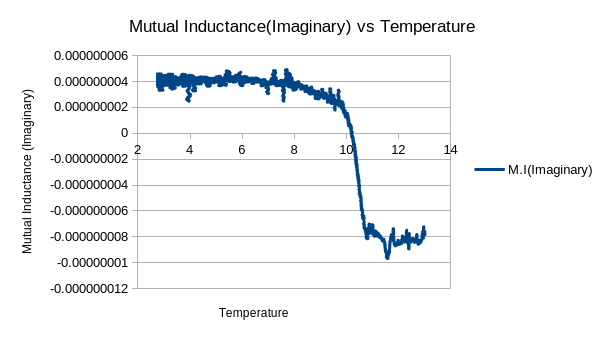
\includegraphics[width=11cm]{plot1.png}
	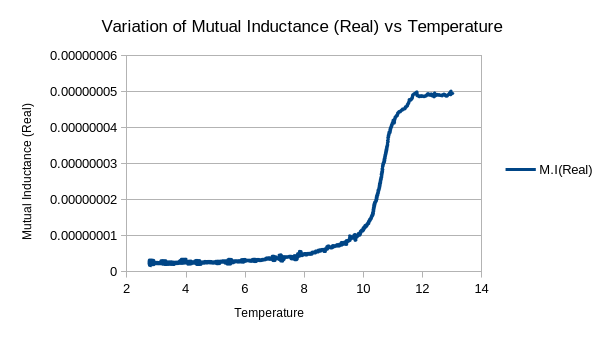
\includegraphics[width=11cm]{plot2.png}\\
	Plot of Mutual Inductance versus the temperature of both parts.
\end{center}
	We are getting the critical temperature of 11.572 K. What is more surprising is that there is some deviation in the real and imaginary values, and in the imaginary part, the mutual inductance didn't rise back up. This might be because the device didn't capture the  change after 14 K, after which it might have risen.
	\\We also didn't analyse the cooling data as it had a lot of fluctuations in temperature. 
	\section*{Result}
	\begin{enumerate}
		\item The Resistance of the coil is 0.292 $\pm$0.001 $\Omega$
		\item The Inductance of the coil is 12 $\pm$ 6 $\mu$H
		\item The critical temperature of the given material is 11.572 K
	\end{enumerate}
\end{document}